\begin{frame}{Jonction P-N : mise en contact de deux types de silicium }

\begin{enumerate}
  \item Mise en contact et diffusion
  \begin{itemize}
    \item \textbf{Loi de Fick} : les porteurs majoritaires diffusent.
    \item Les électrons de N vers P, les trous de P vers N
    \item \textbf{Recombinaisons} au voisinage immédiat de l'interface.
  \end{itemize}
  \item La \textbf{zone de déplétion} (ZCE) : zone vidée de ses porteurs libres
  \begin{itemize}
    \item côté N : des ions donneurs positifs non compensés
    \item côté P : des ions accepteurs négatifs non compensés
    \item ZCE : région dépourvue de porteurs mobiles mais chargée électriquement.
  \end{itemize}

  \item \textbf{Champ interne} et barrière de potentiel
  \begin{itemize}
    \item un champ électrique interne $\vec{E}$, orienté de N vers P, qui s'oppose à la diffusion.
  \end{itemize}

  \item Équilibre dynamique :
  \begin{itemize}
    \item Une barrière de potentiel $V_0$ s'établit (environ 0,7 V pour le silicium).
    \item Le courant de diffusion (dû au gradient) équilibre exactement le courant de conduction (dû  au champ électrique).
    \item Le niveau de Fermi $E_F$ devient continu à travers tout le matériau.
  \end{itemize}
\end{enumerate}
\end{frame}

%\begin{frame}{Jonction P-N : polarisation }
%
% \begin{enumerate}
%   \item Polarisation directe
%   \begin{itemize}
%     \item + côté P, - côté N.
%     \begin{itemize}
%       \item La tension externe s'oppose au champ interne :
%       \item la barrière de potentiel diminue. la ZCE se rétrécit
%       \item la diffusion des majoritaires redevient dominante
%       \item le courant croît exponentiellement avec V.
%     \end{itemize}
%     \item Loi de Shockley : $I = I_0(e^{V/V_T} - 1)$
%   \end{itemize}
%   \item Polarisation inverse
%   \begin{itemize}
%     \item champ externe renforce le champ interne
%     \item la ZCE s'élargit
%     \item très faible courant
%   \end{itemize}
% \end{enumerate}
% \end{frame}

\begin{frame}{Jonction P-N : polarisation}
    \begin{columns}[T]  % [T] aligne en haut, [c] centré, [b] en bas
        \begin{column}{0.5\textwidth}  % Colonne de gauche (50% de la largeur)
          \begin{enumerate}
            \item Polarisation directe
            \begin{itemize}
              \item + côté P, - côté N.
              \begin{itemize}
                \item La tension externe s'oppose au champ interne.
                \item la barrière de potentiel diminue. la ZCE se rétrécit.
                \item la diffusion des majoritaires redevient dominante.
                \item le courant croît exponentiellement avec V.
              \end{itemize}
              \item Loi de Shockley : $I = I_0(e^{V/V_T} - 1)$
            \end{itemize}
            \item Polarisation inverse
            \begin{itemize}
              \item champ externe renforce le champ interne
              \item la ZCE s'élargit
              \item très faible courant
            \end{itemize}
          \end{enumerate}
        \end{column}

        \begin{column}{0.5\textwidth}  % Colonne de droite (50% de la largeur)
            \centering
            \includesvg[width=\textwidth, height=0.7\textheight, keepaspectratio]{./images/jonction_1}
            % ou avec des dimensions fixes :
            % \includesvg[width=5cm, height=5cm]{chemin/vers/votre_fichier}
        \end{column}
    \end{columns}
\end{frame}

\begin{frame}{Transistor bipolaire : structure}
  \begin{columns}[T]  % [T] aligne en haut, [c] centré, [b] en bas
        \begin{column}{0.45\textwidth}  % Colonne de gauche (50% de la largeur)
          \begin{itemize}
            \item Deux jonctions PN dos-à-dos : type NPN ou PNP
            \item Trois régions : émetteur, base, collecteur
            \item Base fine et faiblement dopée
            \item Jonction émetteur-base polarisée en direct
            \item Jonction base-collecteur polarisée en inverse
            \item Effet transistor : le courant de base contrôle le courant de collecteur
          \end{itemize}
        \end{column}

        \begin{column}{0.55\textwidth}  % Colonne de droite (50% de la largeur)
            \centering
            \includegraphics[scale=0.18]{./images/bipolar.jpg}
        \end{column}
    \end{columns}
\end{frame}

\begin{frame}{Transistor bipolaire : fonctionnement}
\begin{itemize}
    \item Gain en courant $\beta = I_C / I_B$ (typiquement 50 à 300)
    \item Régime actif : amplification (usage analogique)
    \item Régime saturé : interrupteur fermé (les 2 jonctions en direct)
    \item Régime bloqué : interrupteur ouvert (les 2 jonctions en inverse)
    \item Relation fondamentale : $I_E = I_B + I_C$
    \item Applications : amplification, commutation, logique TTL
\end{itemize}
\end{frame}
%
% \begin{frame}{Transistor bipolaire : fonctionnement}
%   \begin{itemize}
%   \item  \textbf{Injection} : La polarisation en direct de la jonction EB "pousse" les trous (porteurs majoritaires de l'émetteur P) à travers la jonction pour les injecter dans la base N.
%   \item \textbf{Traversée de la base} : Comme la base est très fine et faiblement dopée, la grande majorité des trous injectés ne trouvent pas d'électrons avec lesquels se recombiner. Ils diffusent donc à travers la base jusqu'à la jonction CB.
%   \item \textbf{Collecte} : La jonction CB étant polarisée en inverse, elle crée un champ électrique intense dans sa zone de déplétion. Ce champ "aspire" immédiatement les trous qui arrivent de la base et les accélère vers le collecteur P.
%   \item \textbf{Recombinaison} (Courant de base) : Une très petite fraction des trous (typiquement 1 \% à 5 \%) se recombine avec les électrons dans la base. Pour maintenir la neutralité électrique, le circuit de base doit fournir continuellement de nouveaux électrons, ce qui constitue le faible courant de base.
%   \end{itemize}
% \end{frame}

\begin{frame}{Transistors MOS (nmos)}
  \begin{columns}[c] % [T] aligne en haut, [c] centré, [b] en bas
    \begin{column}{0.5\textwidth}  % Colonne de gauche (50% de la largeur)
      \begin{itemize}
        \item Transistor à \textbf{effet de champ} (FET) à canal N, constitué d’un substrat P, de deux zones N+ (Source et Drain) et d’une grille isolée par un oxyde ($SiO_2$).
        \item Commande \textbf{par la tension} grille-source $V_{GS}$
        \item Création un canal conducteur (ou non) d’électrons entre Source et Drain.
        \item Inconvénient : un inverseur NMOS utilise une résistance de pull-up.
      \end{itemize}
    \end{column}

    \begin{column}{0.5\textwidth}  % Colonne de droite (50% de la largeur)
        \begin{center}
          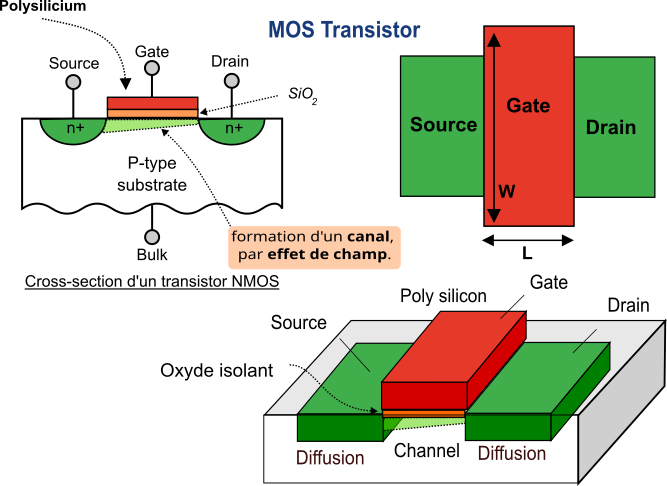
\includegraphics[scale=0.43]{./images/nmos_diagram.png}
        \end{center}
    \end{column}
    \end{columns}
\end{frame}



%===================================================

\begin{frame}{Le procédé de photolithographie}

\begin{columns}[T,onlytextwidth]

  % ---- Colonne de gauche : points clés ----
  \begin{column}{0.47\textwidth}
    \footnotesize
    \begin{itemize}\setlength{\itemsep}{3pt}
      \item \textbf{Principe} : transférer un motif géométrique d'un masque vers une résine photosensible déposée sur une plaquette (\emph{wafer})
      \item \textbf{Dépôt} : enduction centrifuge (\emph{spin coating}) d'un film uniforme
      \item \textbf{Insolation} : exposition UV à travers un masque optique portant le motif
      \item \textbf{Développement} : dissolution sélective des zones exposées (résine positive) ou non exposées (négative)
      \item \textbf{Gravure} : transfert du motif dans le substrat (voie humide ou plasma)
      \item \textbf{Retrait} de la résine (\emph{stripping})
      \item Résolution limitée par la diffraction $\Rightarrow$ UV profond, immersion, EUV
    \end{itemize}
  \end{column}

  % ---- Colonne de droite : schéma ----
  \begin{column}{0.51\textwidth}
    \centering
    \includegraphics[width=\textwidth]{./images/photolitho_v2.pdf}
  \end{column}

\end{columns}

\end{frame}


\begin{frame}{ASML : le leader de la photo-lithographie}
  \begin{columns}
    \begin{column}{0.7\textwidth}
      \begin{center}
        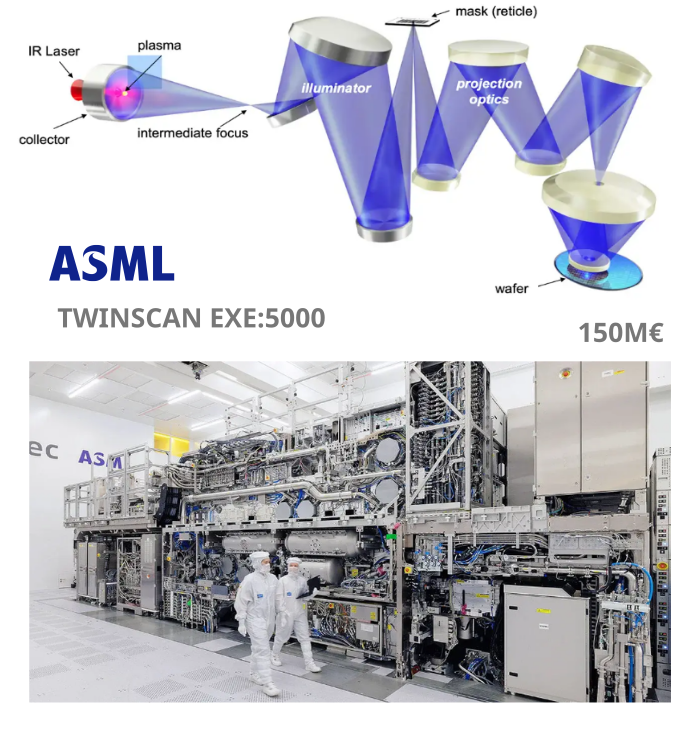
\includegraphics[scale=0.37]{./images/asml.png}
      \end{center}
    \end{column}
    \begin{column}{0.3\textwidth}
      \begin{center}
        \includegraphics[scale=0.4]{./images/ic_3d.jpg}
      \end{center}
    \end{column}
  \end{columns}
\end{frame}
